\chapter{Experiments and Results}
\label{chap:4}
%
In this chapter experiments, made by using different simulation setups, are described. The number of experiments for each trajectory class and for each map is done. Results were analyzed separately and then compared.

\section{Vehicle is Moving Through X-Intersection}

Every time we start belief update calculation we have to initialize the value of belief at the very first time step. When the testing map is X-intersection (Figure~\ref{fig:Xint}), from its' starting position, which is $x_0,y_0 = (14.5, 2.0)$ car can go to any direction it wants: right, straight or left. There are equal chances that car will go to any direction, so initial belief set to be equal for each direction $b_0 = (0.333, 0.333, 0.333)$

\begin{figure}[h]
	\centering  	
	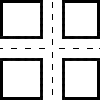
\includegraphics[width=4cm]{img/X-int.jpg}
	\caption{X-intersection map}
	\label{fig:Xint}    
\end{figure}

\subsection{Moving to the Right Direction}

The testing trajectory of going to right looks as it is shown as a red line in Figure~\ref{fig:right}.

\begin{figure}[h]
	\centering  	
	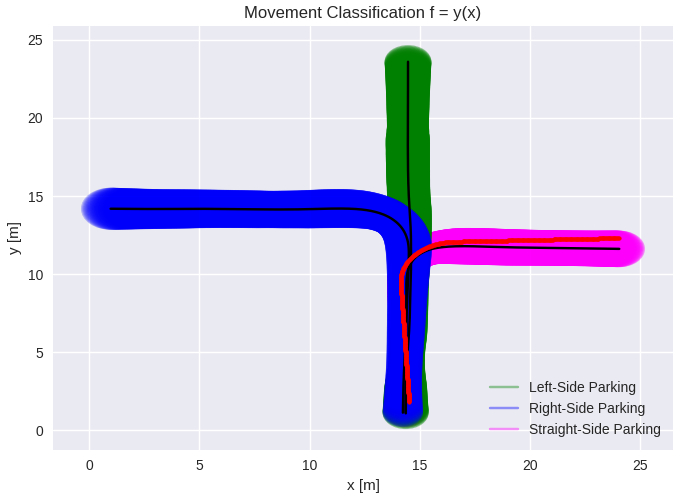
\includegraphics[width=10cm]{img/right_org.jpg}
	\caption{Testing Trajectory (red) of going to the right}
	\label{fig:right}    
\end{figure}

At first, the prediction making was checked for all trajectory, when it has 10-time steps. Results are in Figure~\ref{fig:rightPrediction}. 

\begin{figure}[h]
	\centering  	
	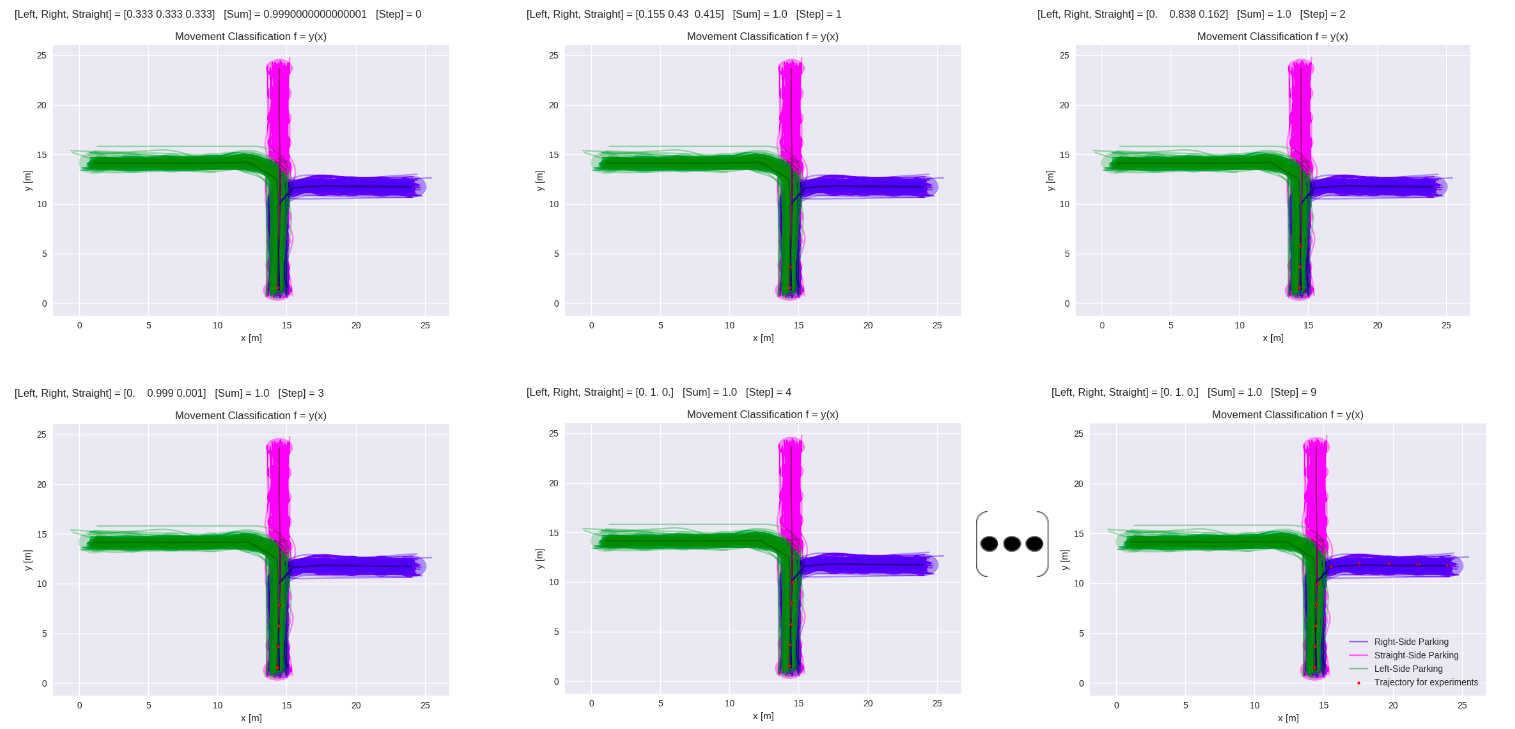
\includegraphics[width=18cm]{img/0_prediction_right.PNG}
	\caption{Prediction making for trajectory which goes to the right. Trajectory has 10-time steps}
	\label{fig:rightPrediction}    
\end{figure}

From the series of plots, we can see that in the 7th step belief that direction is right equals to 1. In Figure~\ref{fig:CompareRight} is shown how beliefs are changing over time. Left graph of the Figure~\ref{fig:CompareRight} shows belief changes when trajectory has 10 points and for better visibility, there was added one more graph on the right, where is the same trajectory, just it was interpolated 100 times instead of 10.

\begin{figure}[h]
	\centering  	
	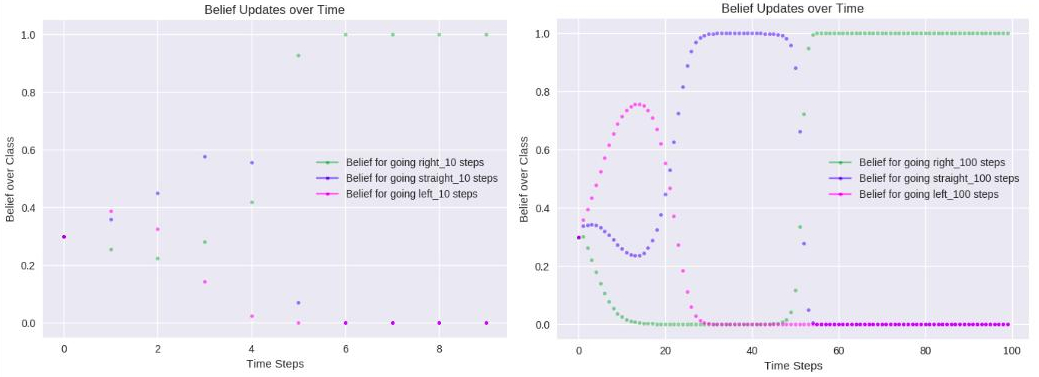
\includegraphics[width=15cm]{img/10_100_compared_right.jpg}
	\caption{Belief changes over time. For trajectory with 10 steps on the left, for trajectory with 100 steps on the right. Trajectory direction is right}
	\label{fig:CompareRight}    
\end{figure}

To be able to see how belief is changing over time withing different trajectories and compare if there are the same results at the same steps in the same movement class, we plotted 10 random trajectories going to the right. Results are shown in Figure~\ref{fig:10Rights}.

\begin{figure}[h]
	\centering  	
	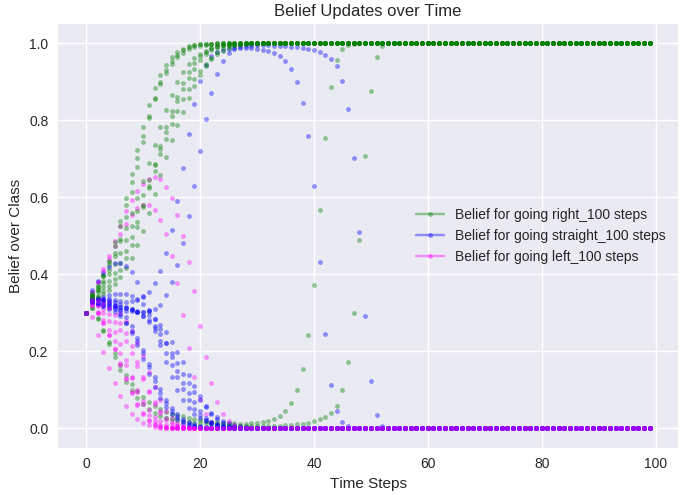
\includegraphics[width=10cm]{img/10_rights.jpg}
	\caption{Belief changes over time for different trajectories which belong to the same movement class. Trajectories have 100 time steps. Trajectory direction is right}
	\label{fig:10Rights}    
\end{figure}

From the Figure~\ref{fig:10Rights} it is possible to see that some trajectories have a better time for being sure to which direction car is moving and some of them have a worse time than others. Next two figures will show trajectories which have "the best" (Figure~\ref{fig:RightGood}) and "the worst" (Figure~\ref{fig:RightBad}) times in the movement prediction.

\begin{figure}[h]
	\centering  	
	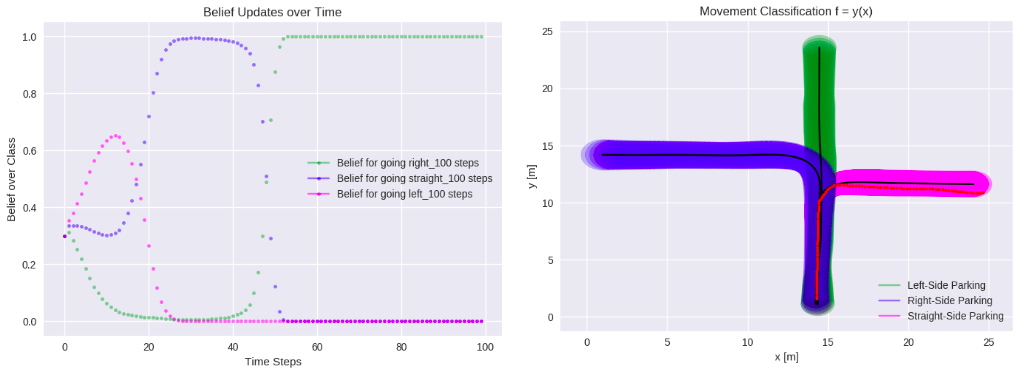
\includegraphics[width=15cm]{img/bad_right_tr.jpg}
	\caption{Belief over time changing (left image) and image of testing trajectory (right image). Trajectories have 100 time steps. Trajectory direction is right}
	\label{fig:RightBad}    
\end{figure}

\begin{figure}[h]
	\centering  	
	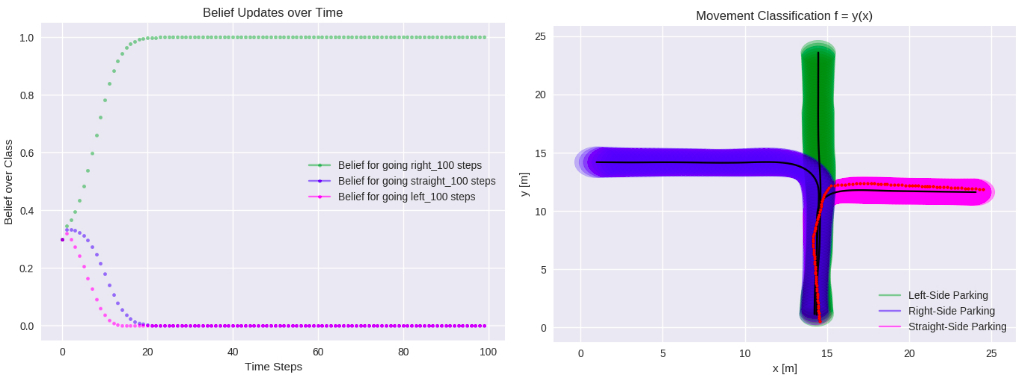
\includegraphics[width=15cm]{img/good_right_tr.jpg}
	\caption{Belief over time changing (left image) and image of testing trajectory (right image). Trajectories have 100 time steps. Trajectory direction is right}
	\label{fig:RightGood}    
\end{figure}

By looking at Figure~\ref{fig:RightBad}, "the worst" results can be explained by the position of the trajectory: it is close to all means, so it is natural that precise of prediction making can be disturbed in this case. \\
By looking at Figure~\ref{fig:RightGood} and "good" results we can also make an assumption that trajectory is not on the means of classes and due to that precise of prediction making is better in this case. 

\subsection{Moving Straight}

The testing trajectory of going straight looks as it is shown as a red line in Figure~\ref{fig:straight}.

\begin{figure}[h]
	\centering  	
	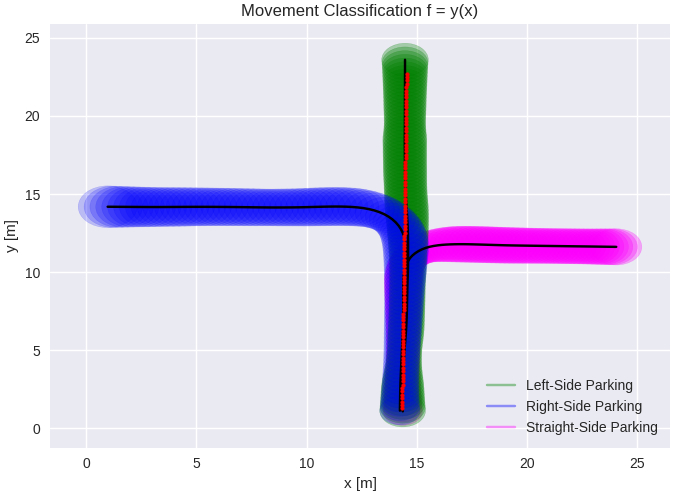
\includegraphics[width=10cm]{img/straight_org.jpg}
	\caption{Testing Trajectory (red) of going straight}
	\label{fig:straight}    
\end{figure}

At first, the prediction making was checked for all trajectory, when it has 10-time steps. Results are in Figure~\ref{fig:straightPrediction}. 

\begin{figure}[h]
	\centering  	
	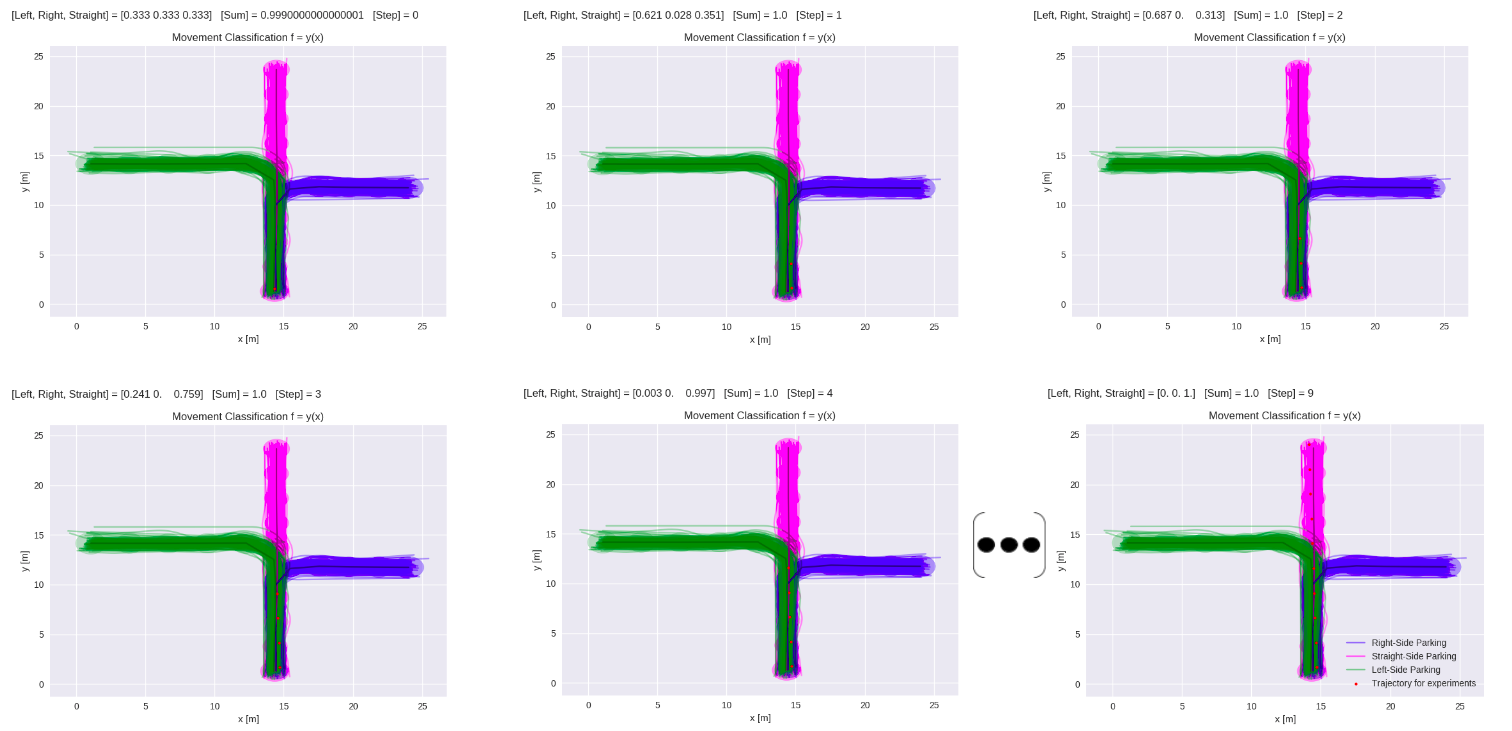
\includegraphics[width=18cm]{img/0_prediction_straight.PNG}
	\caption{Prediction making for trajectory which goes straight. Trajectory has 10-time steps}
	\label{fig:straightPrediction}    
\end{figure}

From the series of plots, we can see that in the 4th step belief that direction is straight is equal to $0.983$. In Figure~\ref{fig:CompareStraight} is shown how beliefs are changing over time. Left graph of the Figure~\ref{fig:CompareStraight} shows belief changes when trajectory has 10 points and for better visibility, there was added one more graph on the right, where is the same trajectory, just it was interpolated 100 times instead of 10.

\begin{figure}[h]
	\centering  	
	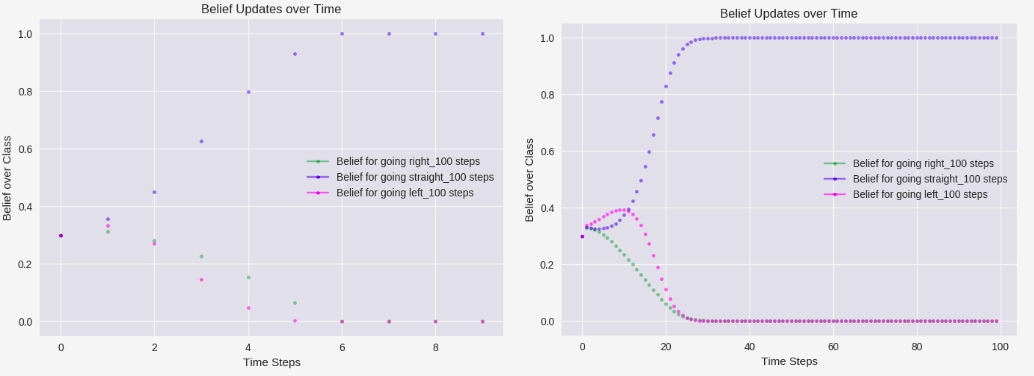
\includegraphics[width=15cm]{img/10_100_compared_straight.jpg}
	\caption{Belief changes over time. For trajectory with 10 steps on the left, for trajectory with 100 steps on the right. Trajectory direction is straight}
	\label{fig:CompareStraight}    
\end{figure}

To be able to see how belief is changing over time withing different trajectories and compare if there are the same results at the same steps in the same movement class, we plotted 10 random trajectories going straight. Results are shown in Figure~\ref{fig:10Straight}.

\begin{figure}[h]
	\centering  	
	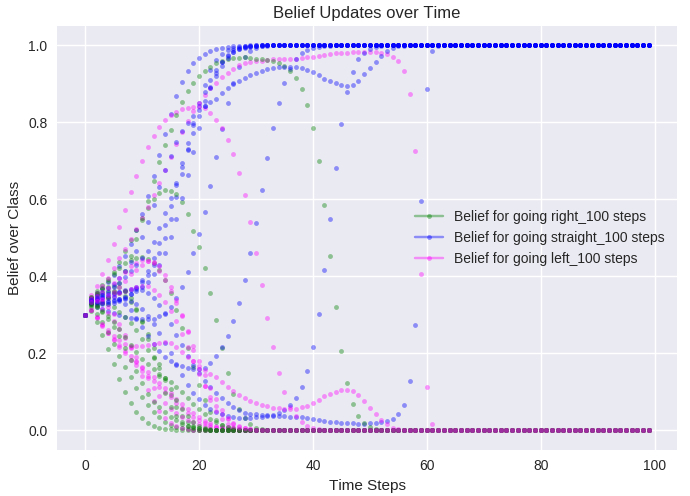
\includegraphics[width=10cm]{img/10_straights.jpg}
	\caption{Belief changes over time for different trajectories which belong to the same movement class. Trajectories have 100 time steps. Trajectory direction is straight}
	\label{fig:10Straight}    
\end{figure}

From the Figure~\ref{fig:10Straight} it is possible to see that some trajectories have a better time for being sure to which direction car is moving and some of them have a worse time than others. Next two figures will show trajectories which have "the best" (Figure~\ref{fig:StraightGood}) and "the worst" (Figure~\ref{fig:StraightBad}) times in the movement prediction.

\begin{figure}[h]
	\centering  	
	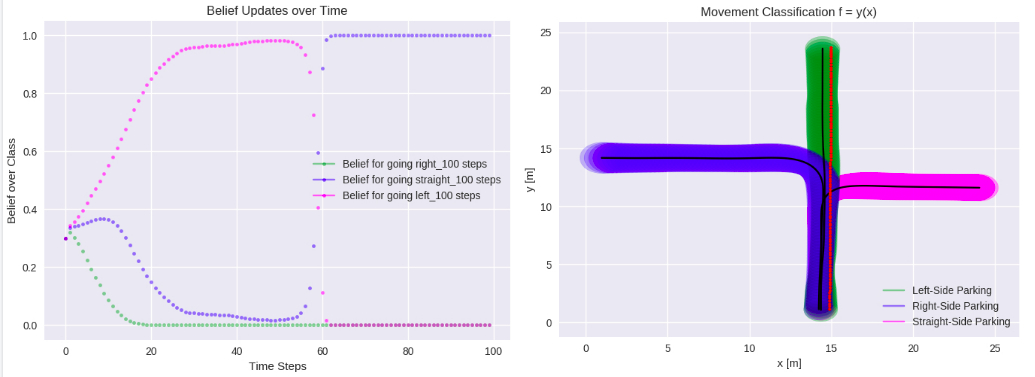
\includegraphics[width=15cm]{img/bad_straight_tr.jpg}
	\caption{Belief over time changing (left image) and image of testing trajectory (right image). Trajectories have 100 time steps. Trajectory direction is straight}
	\label{fig:StraightBad}    
\end{figure}

\begin{figure}[h]
	\centering  	
	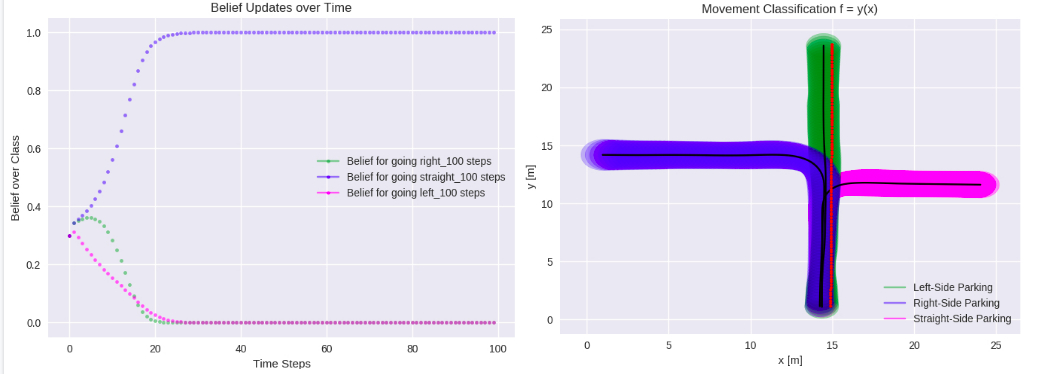
\includegraphics[width=15cm]{img/good_straight_tr.jpg}
	\caption{Belief over time changing (left image) and image of testing trajectory (right image). Trajectories have 100 time steps. Trajectory direction is straight}
	\label{fig:StraightGood}    
\end{figure}

By looking at Figure~\ref{fig:StraightBad}, "the worst" results can be explained by the position of the trajectory: it is closer to standard deviation values of left class mean, this could be the case, why prediction is that car is going to the left, until it is sure that it is not going to the left. \\
By looking at Figure~\ref{fig:StraightGood} and "good" results we can also make an assumption that trajectory and coordinates at each time step is closer to mean and it is in the range of standard deviation of straight mean.

By looking into separate results of class straight one more very interesting case was noticed. Here (Figure~\ref{fig:InterestingGood}) prediction is correct from the very first steps, but the changing of dynamics of prediction is interesting.  This dynamics might be explained by car movement trajectory (it is not moving exactly straight, it is making some turning, which can be the reason of this result).

\begin{figure}[h]
	\centering  	
	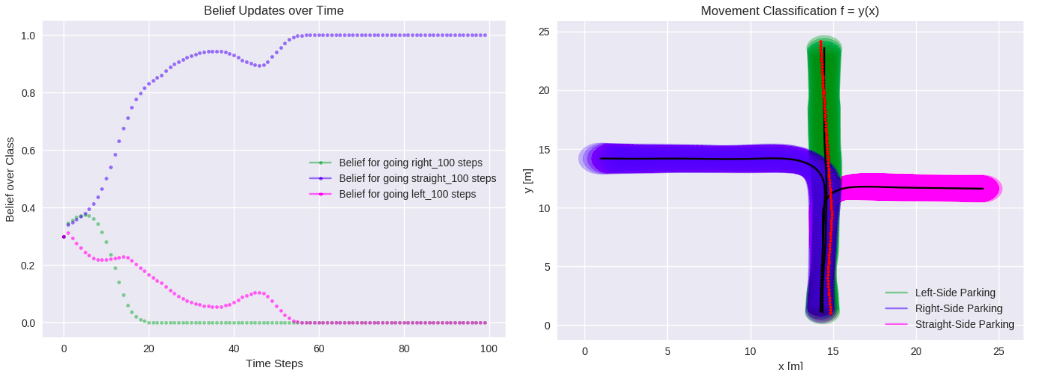
\includegraphics[width=15cm]{img/interesting_straight_tr.jpg}
	\caption{Belief over time changing (left image) and image of testing trajectory (right image). Trajectories have 100 time steps. Trajectory direction is straight}
	\label{fig:InterestingGood}    
\end{figure}

\subsection{Moving to the Left Direction}

The testing trajectory of going to the left looks as it is shown as a red line in Figure~\ref{fig:left}.

\begin{figure}[h]
	\centering  	
	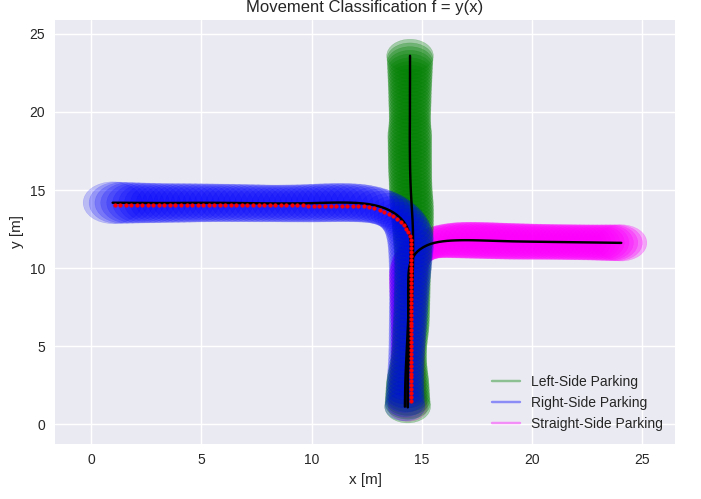
\includegraphics[width=10cm]{img/left_org.jpg}
	\caption{Testing Trajectory (red) of going to the left}
	\label{fig:left}    
\end{figure}

At first, the prediction making was checked for all trajectory, when it has 10-time steps. Results are in Figure~\ref{fig:leftPrediction}. 

\begin{figure}[h]
	\centering  	
	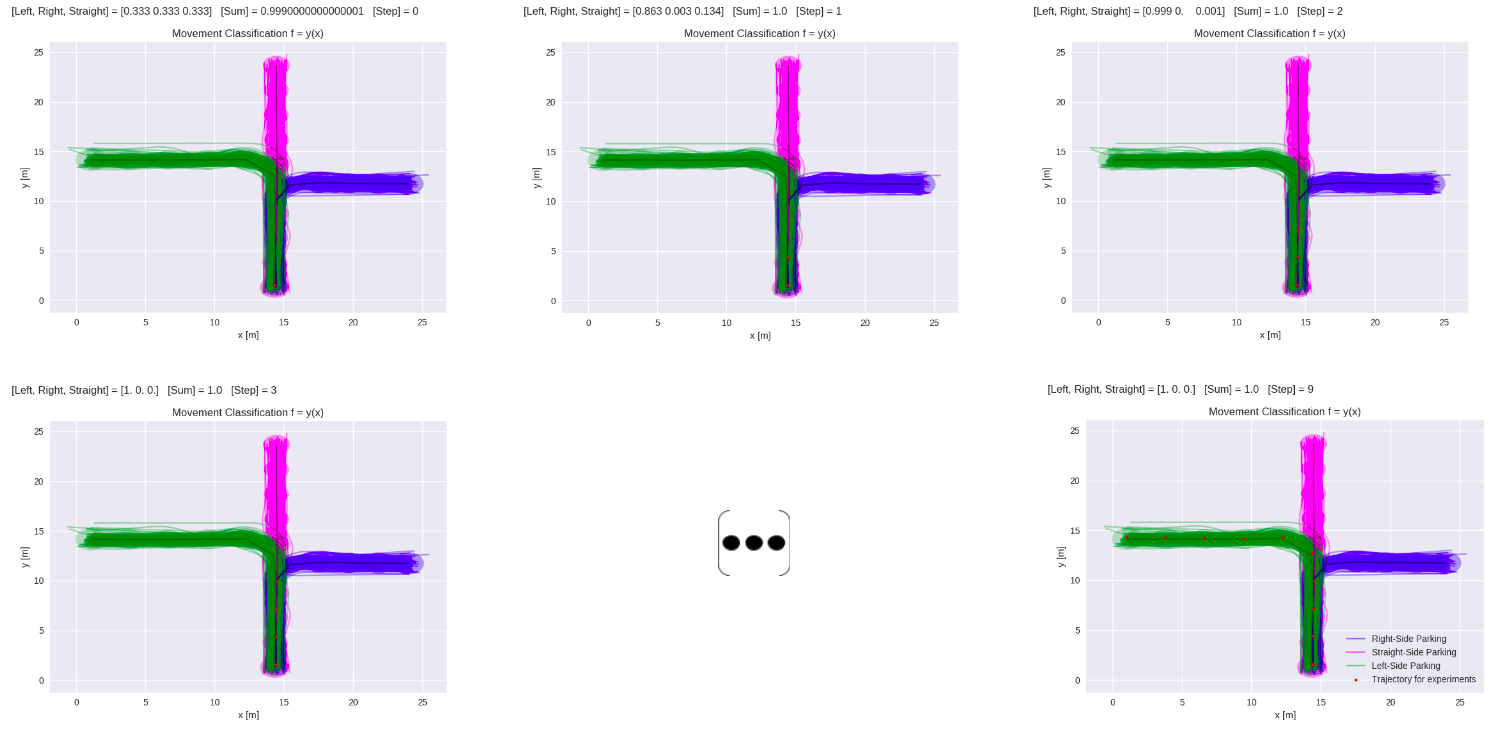
\includegraphics[width=18cm]{img/0_prediction_left.PNG}
	\caption{Prediction making for trajectory which goes left. Trajectory has 10-time steps}
	\label{fig:leftPrediction}    
\end{figure}

From the series of plots, we can see that in the 3rd step belief that direction is left is equal to $0.935$. In Figure~\ref{fig:CompareLeft} is shown how beliefs are changing over time. Left graph of the Figure~\ref{fig:CompareLeft} shows belief changes when trajectory has 10 points and for better visibility, there was added one more graph on the right, where is the same trajectory, just it was interpolated 100 times instead of 10.

\begin{figure}[h]
	\centering  	
	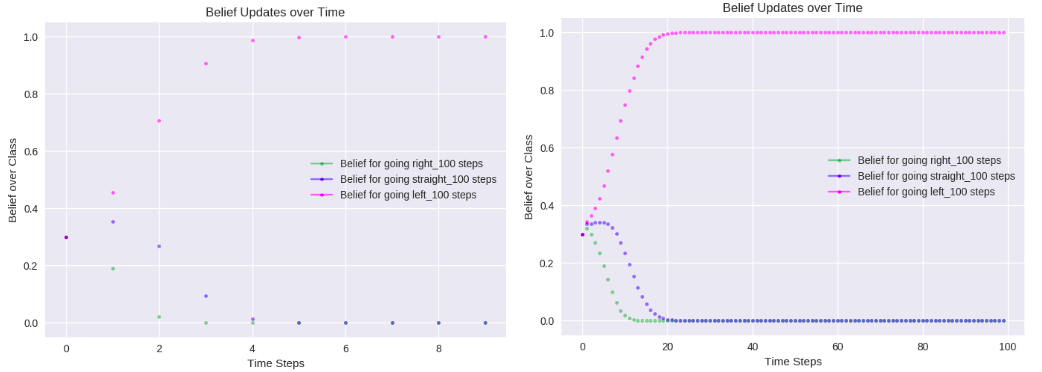
\includegraphics[width=15cm]{img/10_100_compared_left.jpg}
	\caption{Belief changes over time. For trajectory with 10 steps on the left, for trajectory with 100 steps on the right. Trajectory direction is left}
	\label{fig:CompareLeft}    
\end{figure}

To be able to see how belief is changing over time withing different trajectories and compare if there are the same results at the same steps in the same movement class, we plotted 10 random trajectories going straight. Results are shown in Figure~\ref{fig:10Left}.

\begin{figure}[h]
	\centering  	
	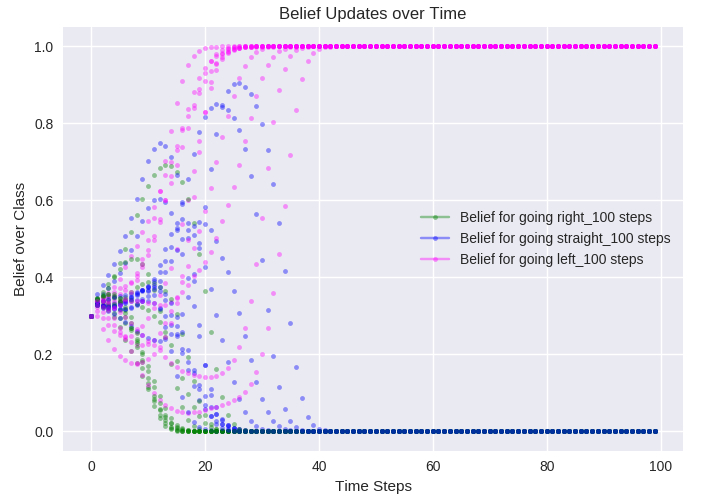
\includegraphics[width=10cm]{img/10_lefts.jpg}
	\caption{Belief changes over time for different trajectories which belong to the same movement class. Trajectories have 100 time steps. Trajectory direction is left}
	\label{fig:10Left}    
\end{figure}

From the Figure~\ref{fig:10Left} it is possible to see that some trajectories have a better time for being sure to which direction car is moving and some of them have a worse time than others. Next two figures will show trajectories which have "the best" (Figure~\ref{fig:LeftGood}) and "the worst" (Figure~\ref{fig:LeftBad}) times in the movement prediction.

\begin{figure}[h]
	\centering  	
	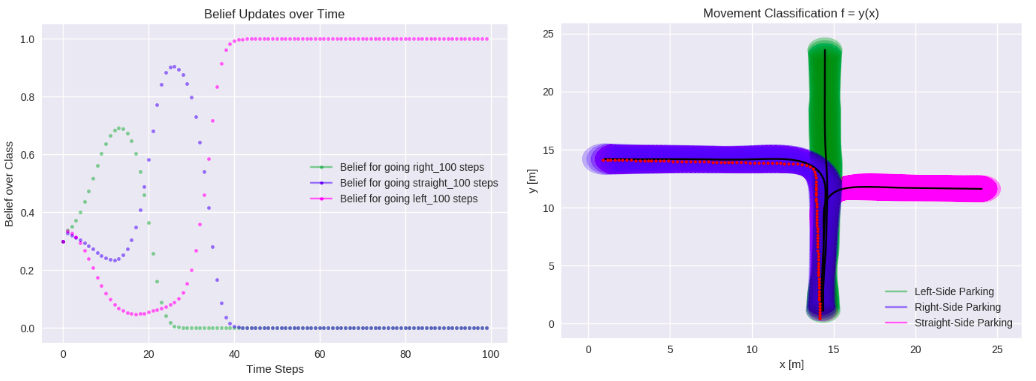
\includegraphics[width=15cm]{img/bad_left_tr.jpg}
	\caption{Belief over time changing (left image) and image of testing trajectory (right image). Trajectories have 100 time steps. Trajectory direction is left}
	\label{fig:LeftBad}    
\end{figure}

\begin{figure}[h]
	\centering  	
	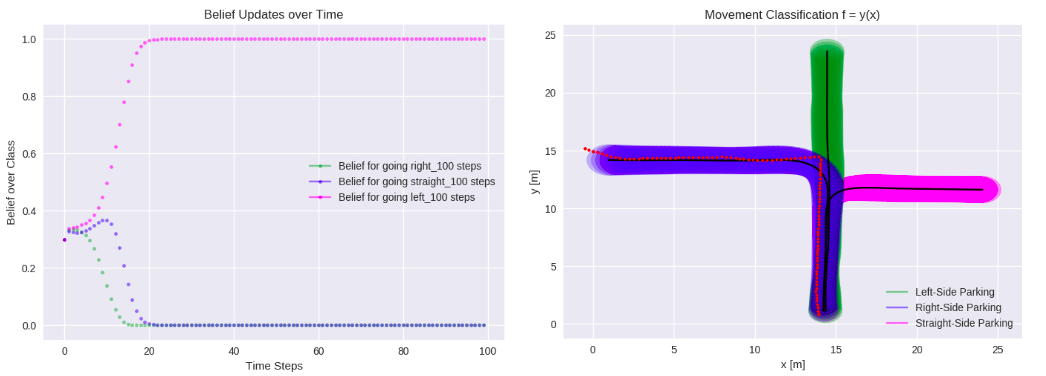
\includegraphics[width=15cm]{img/good_left_tr.jpg}
	\caption{Belief over time changing (left image) and image of testing trajectory (right image). Trajectories have 100 time steps. Trajectory direction is left}
	\label{fig:LeftGood}    
\end{figure}

\textcolor{red}{TO THINK WHY IT IS DIFFER}


\section{Vehicle is Moving Through T-Intersection}

In this section results of simulation setup for T-Intersection (map looks like it is shown in Figure~\ref{fig:Tint}) will be described. As in the case of the map with X-Intersection, starting position of the car is $x_0,y_0 = (14.5, 2.0)$, but in this setup, the car can go only to the left or right, straight direction does not exist in this case. As in the previous case, at the very beginning, initial belief must be set. Since we already know that there is no way that car is going straight (there is no straight from car starting position), we have so-called some prior information. Initial belief for going right and left is calculated by formula $\frac{\# of trajectories going to the right in our database}{\# of trajectories going to the right in our database + \# of trajectories going to the left in our database}$ and $\frac{\# of trajectories going to the left in our database}{\# of trajectories going to the right in our database + \# of trajectories going to the left in our database}$ respectively. After calculation initial belief set to be $b_0 [left, right, straight]= (0.533, 0.467, 0.000)$

\begin{figure}[h]
	\centering  	
	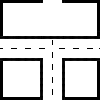
\includegraphics[width=4cm]{img/T-int.jpg}
	\caption{T-intersection map}
	\label{fig:Tint}    
\end{figure}

\subsection{Moving to the Right Direction}

The testing trajectory of going to right looks as it is shown as a red line in Figure~\ref{fig:right_T}.

\begin{figure}[h]
	\centering  	
	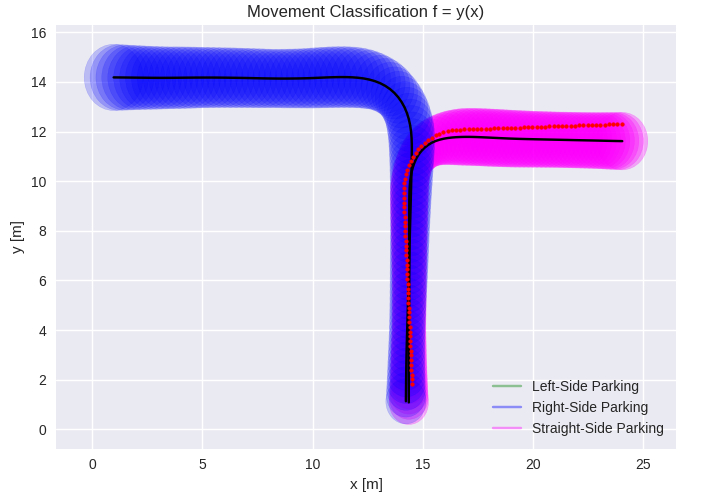
\includegraphics[width=10cm]{img/right_org_T.jpg}
	\caption{Testing Trajectory (red) of going to right}
	\label{fig:right_T}    
\end{figure}

In Figure~\ref{fig:CompareRightT} is shown how beliefs are changing over time. Left graph of the Figure~\ref{fig:CompareRightT} shows belief changes when trajectory has 10 points and for better visibility, there was added one more graph on the right, where is the same trajectory, just it was interpolated 100 times instead of 10.

\begin{figure}[h]
	\centering  	
	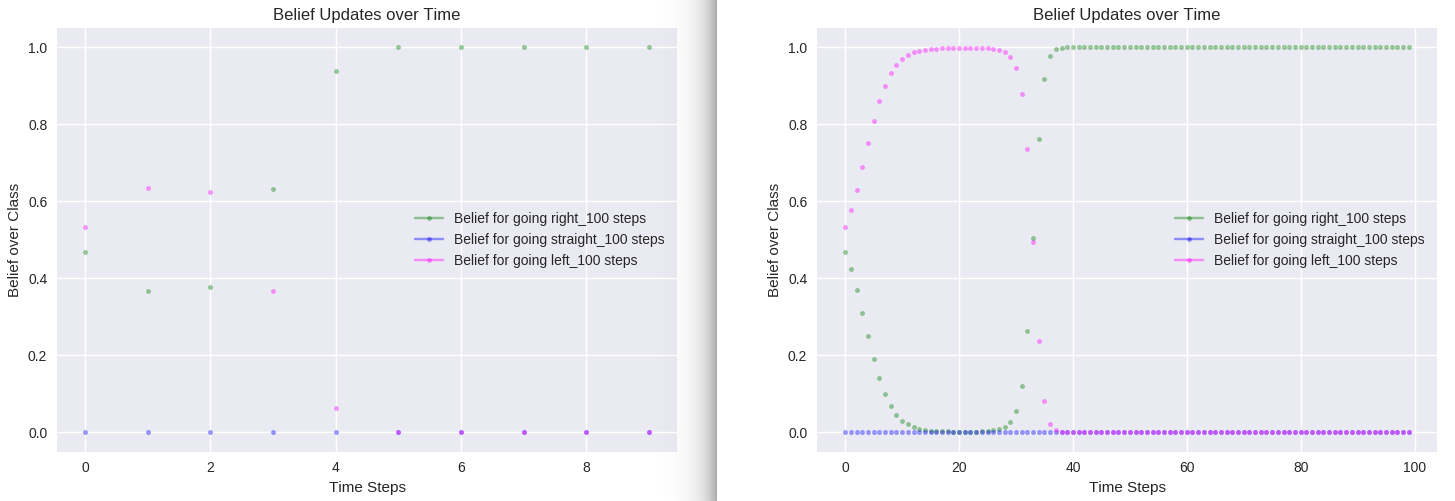
\includegraphics[width=15cm]{img/10_100_compared_right_T.jpg}
	\caption{Belief changes over time. For trajectory with 10 steps on the left, for trajectory with 100 steps on the right. Trajectory direction is right}
	\label{fig:CompareRightT}    
\end{figure}

To be able to see how belief is changing over time withing different trajectories and compare if there are the same results at the same steps in the same movement class, we plotted 10 random trajectories going to the right. Results are shown in Figure~\ref{fig:10RightsT}.

\begin{figure}[h]
	\centering  	
	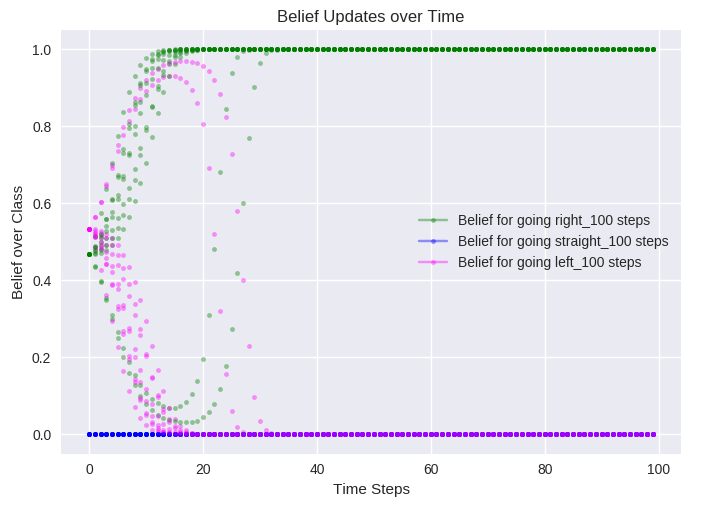
\includegraphics[width=10cm]{img/10Rights_T.jpg}
	\caption{Belief changes over time for different trajectories which belong to the same movement class. Trajectories have 100 time steps. Trajectory direction is right}
	\label{fig:10RightsT}    
\end{figure}

From the Figure~\ref{fig:10RightsT} it is possible to see that correct prediction is made much faster than in case of map with X-Intersection (Figure~\ref{fig:10Rights}).

\subsection{Moving to the Left Direction}

The testing trajectory of going to right looks as it is shown as a red line in Figure~\ref{fig:left_T}.

\begin{figure}[h]
	\centering  	
	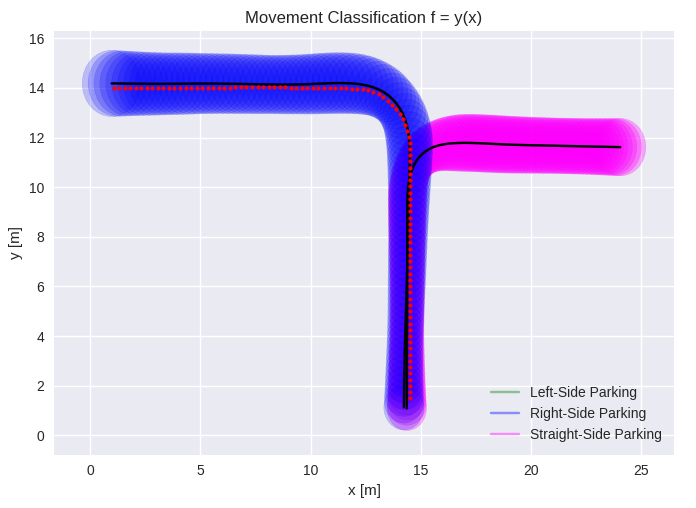
\includegraphics[width=10cm]{img/left_org_T.jpg}
	\caption{Testing Trajectory (red) of going to the left}
	\label{fig:left_T}    
\end{figure}

In Figure~\ref{fig:CompareLeftT} is shown how beliefs are changing over time. Left graph of the Figure~\ref{fig:CompareLeftT} shows belief changes when trajectory has 10 points and for better visibility, there was added one more graph on the right, where is the same trajectory, just it was interpolated 100 times instead of 10.

\begin{figure}[h]
	\centering  	
	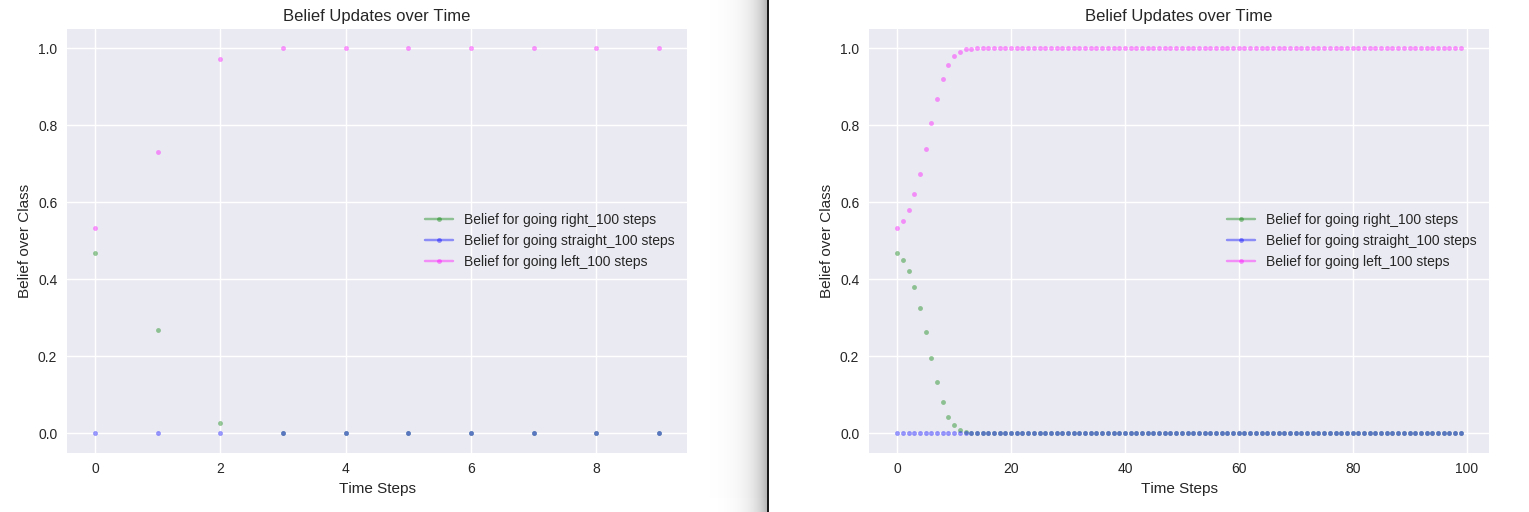
\includegraphics[width=15cm]{img/10_100_compared_left_T.jpg}
	\caption{Belief changes over time. For trajectory with 10 steps on the left, for trajectory with 100 steps on the right. Trajectory direction is left}
	\label{fig:CompareLeftT}    
\end{figure}

To be able to see how belief is changing over time withing different trajectories and compare if there are the same results at the same steps in the same movement class, we plotted 10 random trajectories going to the right. Results are shown in Figure~\ref{fig:10LeftsT}.

\begin{figure}[h]
	\centering  	
	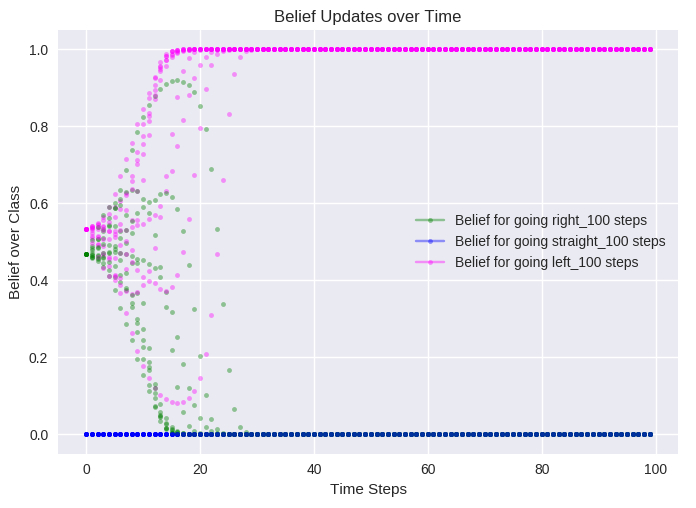
\includegraphics[width=10cm]{img/10_Left_T.jpg}
	\caption{Belief changes over time for different trajectories which belong to the same movement class. Trajectories have 100 time steps. Trajectory direction is left}
	\label{fig:10LeftsT}    
\end{figure}

As we could see from the Figure~\ref{fig:10RightsT}, the same results we can see from Figure~\ref{fig:10LeftsT}: the correct prediction is made much faster than in case of map with X-Intersection. This happened because of prior knowledge.

\section{Results Comparison Before and After Scaling}

 As mentioned before trajectory scaling while updating belief can allow not to make calculations so frequently, but still, keep the same precision of results as having a lot of belief updates. \\
 
 One test on scaling was done having one trajectory interpolated 100 times, at every step in 100-time step trajectory likelihood (formula~\ref{eqn:formula2}) was powered by 0.1 and results were compared with taking every 10th step from the same trajectory, but with calculation as normal. The scaling algorithm is described in Figure~\ref{fig:PseudoScalling}. To show the difference between scaled results and not scaled results two different graphs will be shown for one test.

\subsection{X-Intersection}

X-Intersection has three directions and scaling within all three of them will be shown.

\begin{figure}[h]
	\centering  	
	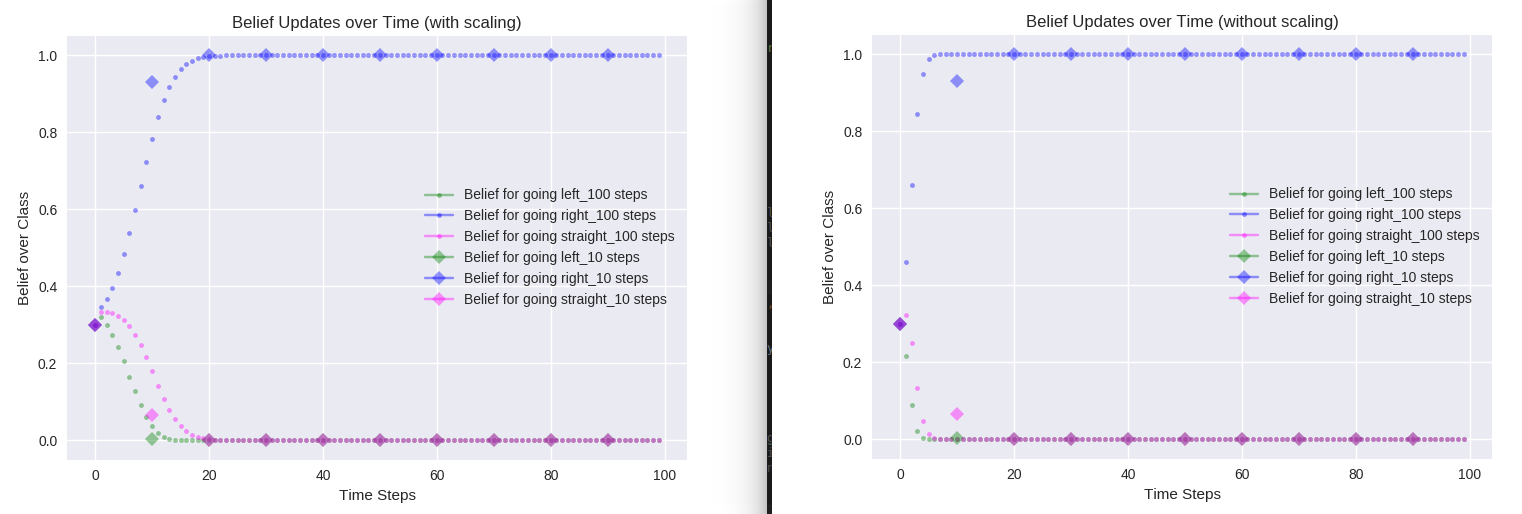
\includegraphics[width=15cm]{img/Scaling_Right_X.jpg}
	\caption{Belief updates using scaling. Direction of the testing trajectory is right}
	\label{fig:ScallingRightX}    
\end{figure}

\begin{figure}[h]
	\centering  	
	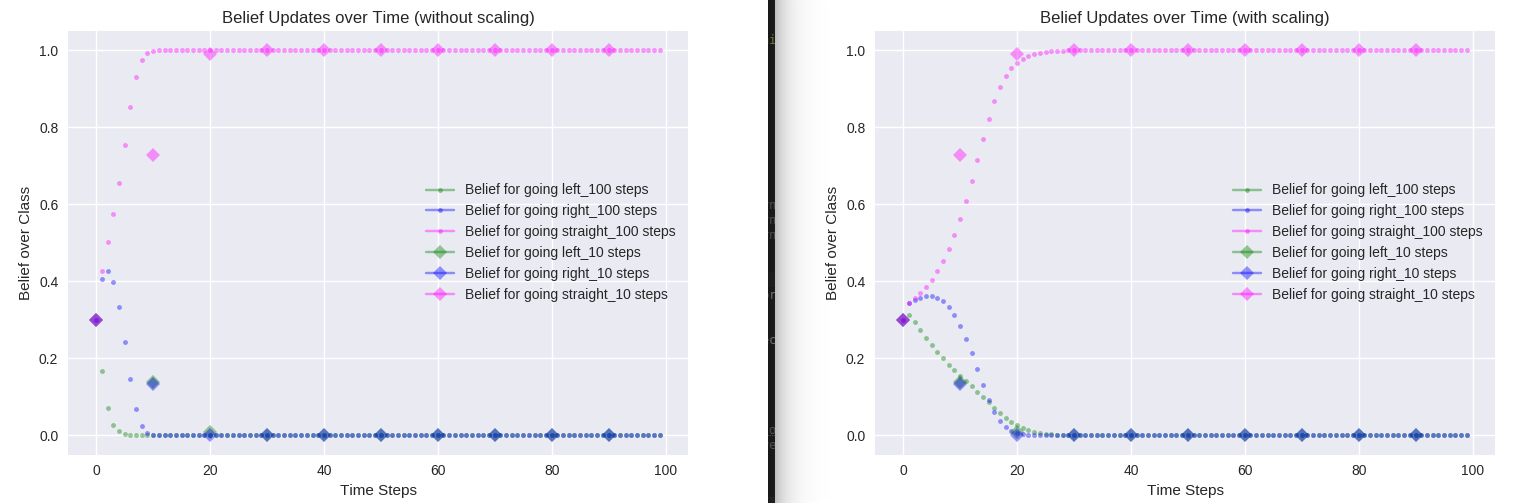
\includegraphics[width=15cm]{img/Scaling_Straight_X.jpg}
	\caption{Belief updates using scaling. Direction of the testing trajectory is straight}
	\label{fig:ScallingStraightX}    
\end{figure}

\begin{figure}[h]
	\centering  	
	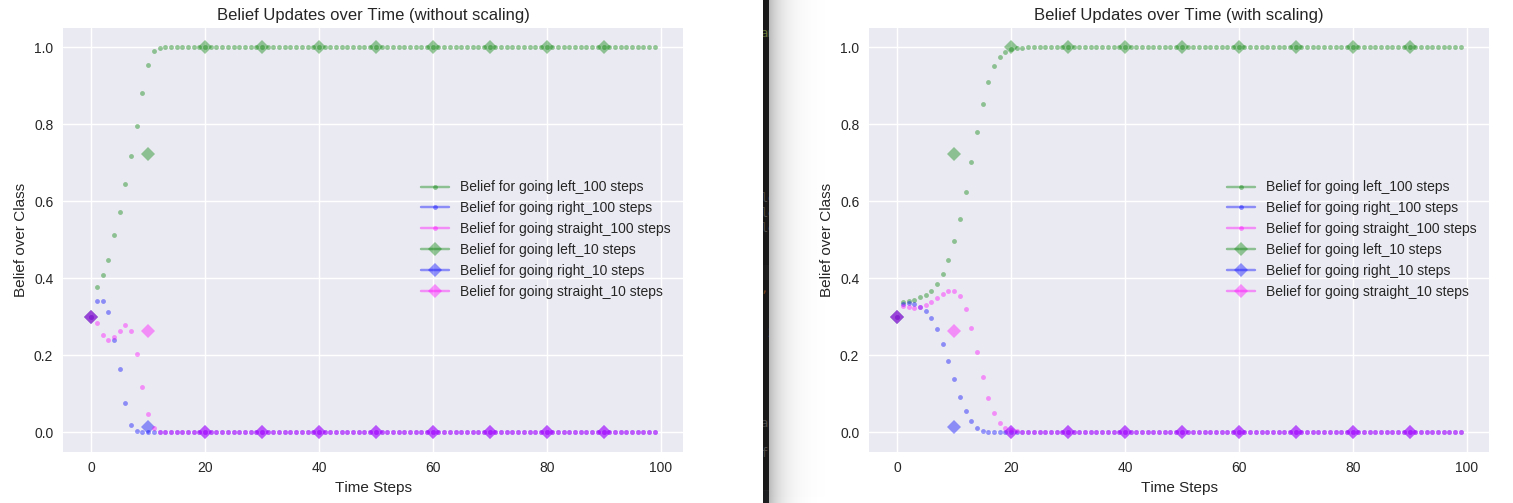
\includegraphics[width=15cm]{img/Scaling_Left_X.jpg}
	\caption{Belief updates using scaling. Direction of the testing trajectory is left}
	\label{fig:ScallingLeftX}    
\end{figure}


\subsection{T-Intersection}

X-Intersection has two directions and scaling within right and left directions will be shown.

\begin{figure}[h]
	\centering  	
	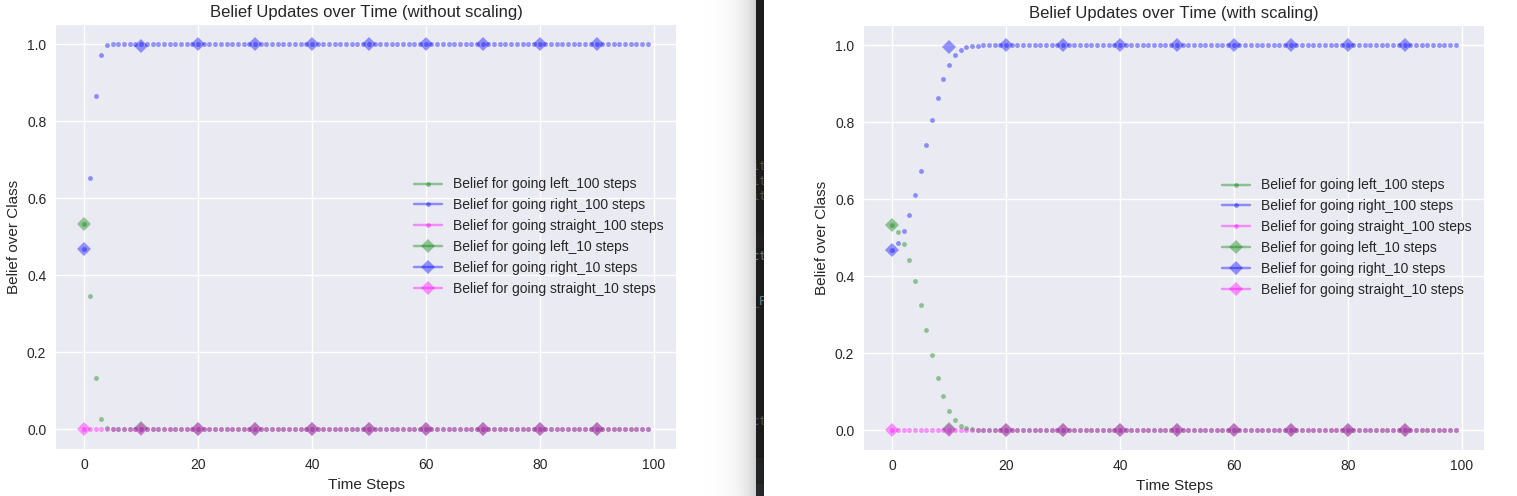
\includegraphics[width=15cm]{img/Scaling_Right_T.jpg}
	\caption{Belief updates using scaling. Direction of the testing trajectory is right}
	\label{fig:ScallingRightT}    
\end{figure}

\begin{figure}[h]
	\centering  	
	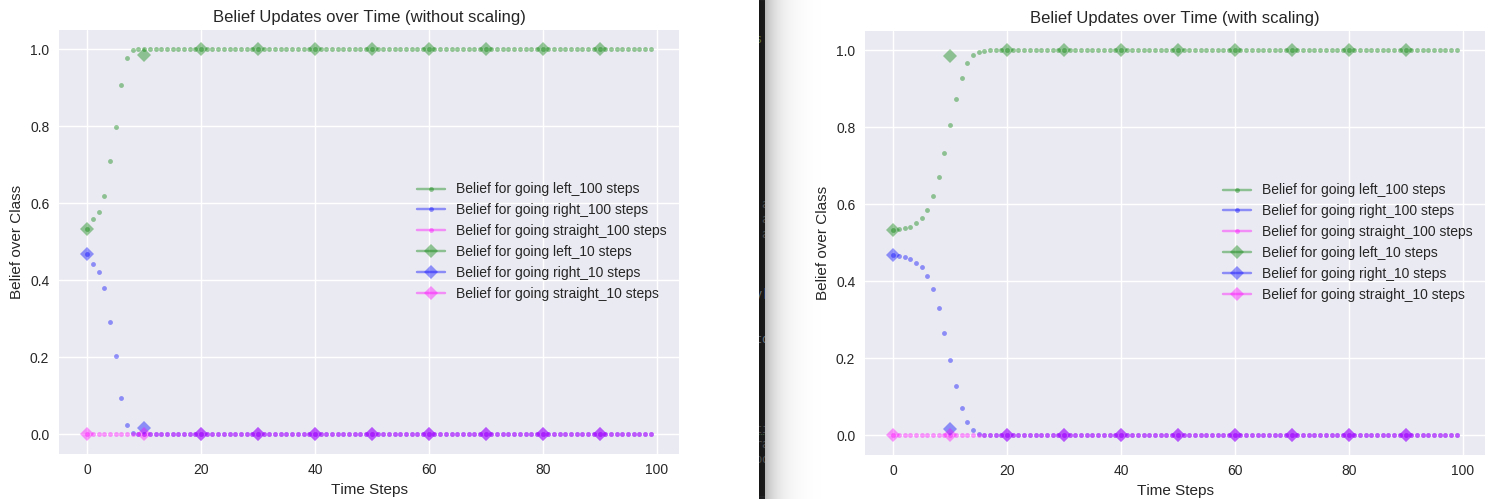
\includegraphics[width=15cm]{img/Scaling_Left_T.jpg}
	\caption{Belief updates using scaling. Direction of the testing trajectory is left}
	\label{fig:ScallingLeftT}    
\end{figure}

\section{Prediction Making in Online Method}

\textcolor{red}{in process}